%!TEX program = xelatex
\documentclass[dvipsnames, svgnames,a4paper,11pt]{article}
% ----------------------------------------------------- 
%	加边框的命令
%	参考:https://tex.stackexchange.com/questions/531559/how-to-add-the-page-border-for-first-two-pages-in-latex
\usepackage{tikz}
\usetikzlibrary{calc}
\usepackage{eso-pic}
\AddToShipoutPictureBG{%
\begin{tikzpicture}[overlay,remember picture]
\draw[line width=0.6pt] % 边框粗细
    ($ (current page.north west) + (0.6cm,-0.6cm) $)
    rectangle
    ($ (current page.south east) + (-0.6cm,0.6cm) $); % 边框位置
\end{tikzpicture}}


\usepackage{xcolor}
\definecolor{c1}{HTML}{086173} % 目录颜色 原版为2752C9 紫灰色535AAA 蓝紫色0B0DB7 深蓝色070F94 湖绿色219394 松石灰绿086173
\definecolor{c2}{HTML}{E20129} % 引用颜色 原版\definecolor{c2}{RGB}{190,20,83} 橙色F24729

\usepackage{ctex}
\usepackage[top=28mm,bottom=28mm,left=15mm,right=15mm]{geometry}
\usepackage{hyperref} 
\hypersetup{
	colorlinks,
	linktoc = section, % 超链接位置,选项有section, page, all
	linkcolor = c1, % linkcolor 目录颜色
	citecolor = c1  % citecolor 引用颜色
}
\usepackage{amsmath,enumerate,multirow,float}
\usepackage{tabularx}
\usepackage{tabu}
\usepackage{subfig}
\usepackage{fancyhdr}
\usepackage{graphicx}
\usepackage{wrapfig}  
\usepackage{physics}
\usepackage{appendix}
\usepackage{amsfonts}

%
\usepackage{tcolorbox}
\tcbuselibrary{skins,breakable}
\newtcolorbox{tbox}[2][]{
    colframe=black!70!,
    breakable,
    enhanced,
	boxrule =0.5pt,
    title = {#2},
    fonttitle = \large\kaishu\bfseries,
	drop fuzzy shadow,
    #1
}
\newtcolorbox[auto counter,number within=section]{question}[1][]{
  top=2pt,bottom=2pt,arc=1mm,
  boxrule=0.5pt,
%   frame hidden,
  breakable,
  enhanced, %跨页后不会显示下边框
  coltitle=c1!80!gray,
  colframe=c1,
  colback=c1!3!white,
  drop fuzzy shadow,
  title={思考题~\thetcbcounter:\quad},
  fonttitle=\bfseries,
  attach title to upper,
  #1
}

% ---------------------------------------------------------------------
%	利用cleveref改变引用格式,\cref是引用命令
\usepackage{cleveref}
\crefformat{figure}{#2{\textcolor{c2}{Figure #1}}#3} % 图片的引用格式
\crefformat{equation}{#2{(\textcolor{c2}{#1})}#3} % 公式的引用格式
\crefformat{table}{#2{\textcolor{c2}{Table #1}}#3} % 表格的引用格式


% ---------------------------------------------------------------------
%	页眉页脚设置
\fancypagestyle{plain}{\pagestyle{fancy}}
\pagestyle{fancy}
\lhead{\kaishu 中山大学物理与天文学院电子技术实验\uppercase\expandafter{\romannumeral1}} % 左边页眉,学院 + 课程
\rhead{\kaishu 实验报告By黄罗琳} % 右边页眉,实验报告标题
\cfoot{\thepage} % 页脚,中间添加页码


% ---------------------------------------------------------------------
%	对目录、章节标题的设置
\renewcommand{\contentsname}{\centerline{\huge 目录}}
\usepackage{titlesec}
\usepackage{titletoc}
% \titleformat{章节}[形状]{格式}{标题序号}{序号与标题间距}{标题前命令}[标题后命令]
\titleformat{\section}{\centering\LARGE\songti}{}{1em}{}

% ---------------------------------------------------------------------
%   listing代码环境设置
\usepackage{listings}
\lstloadlanguages{python}
\lstdefinestyle{pythonstyle}{
backgroundcolor=\color{gray!5},
language=python,
frameround=tftt,
frame=shadowbox, 
keepspaces=true,
breaklines,
columns=spaceflexible,                   
basicstyle=\ttfamily\small, % 基本文本设置,字体为teletype,大小为scriptsize
keywordstyle=[1]\color{c1}\bfseries, 
keywordstyle=[2]\color{Red!70!black},   
stringstyle=\color{Purple},       
showstringspaces=false,
commentstyle=\ttfamily\scriptsize\color{green!40!black},%注释文本设置,字体为sf,大小为smaller
tabsize=2,
morekeywords={as},
morekeywords=[2]{np, plt, sp},
numbers=left, % 代码行数
numberstyle=\it\tiny\color{gray}, % 代码行数的数字字体设置
stepnumber=1,
rulesepcolor=\color{gray!30!white}
}




% ---------------------------------------------------------------------
%	其他设置
\def\degree{${}^{\circ}$} % 角度
\graphicspath{{./images/}} % 插入图片的相对路径
\allowdisplaybreaks[4]  %允许公式跨页 
\usepackage{lipsum}
\usepackage{adjustbox}
%\usepackage{mathrsfs} % 字体
%\captionsetup[figure]{name=Figure} % 图片形式
%\captionsetup[table]{name=Table} % 表格形式
\begin{document}
	
	% 实验报告封面	
	% 顶栏
	\begin{table}
		\renewcommand\arraystretch{1.7}
		\begin{tabularx}{\textwidth}{
				|X|X|X|X
				|X|X|X|X|}
			\hline
			\multicolumn{2}{|c|}{预习报告}&\multicolumn{2}{|c|}{实验记录}&\multicolumn{2}{|c|}{分析讨论}&\multicolumn{2}{|c|}{总成绩}\\
			\hline
			\LARGE25 & & \LARGE25 & & \LARGE30 & & \LARGE80 & \\
			\hline
		\end{tabularx}
	\end{table}
	% ---
	
	% 信息栏
	\begin{table}
		\renewcommand\arraystretch{1.7}
		\begin{tabularx}{\textwidth}{|X|X|X|X|}
			\hline
			年级、专业: & 2022级 物理学 &组号: & D8\\
			\hline
			姓名: &  黄罗琳、王显 & 学号: &22344001、22344002   \\
			\hline
			实验时间: & 2024/5/29 & 教师签名: & \\
			\hline
		\end{tabularx}
	\end{table}
	% ---
	
	% 大标题
	\begin{center}
		\LARGE ET11 \quad 模拟运算放大电路
	\end{center}
	% ---
	
	% 注意事项
	
	% 基本
	\textbf{【实验报告注意事项】}
	\begin{enumerate}
		\item 实验报告由三部分组成:
		\begin{enumerate}
			\item 预习报告:课前认真研读实验讲义,弄清实验原理;实验所需的仪器设备、用具及其使用、完成课前预习思考题;了解实验需要测量的物理量,并根据要求提前准备实验记录表格(可以参考实验报告模板,可以打印)。\textcolor{red}{\textbf{(20分)}}
			\item 实验记录:认真、客观记录实验条件、实验过程中的现象以及数据。实验记录请用珠笔或者钢笔书写并签名(\textcolor{red}{\textbf{用铅笔记录的被认为无效}})。\textcolor{red}{\textbf{保持原始记录,包括写错删除部分,如因误记需要修改记录,必须按规范修改。}}(不得输入电脑打印,但可扫描手记后打印扫描件);离开前请实验教师检查记录并签名。\textcolor{red}{\textbf{(30分)}}
			\item 数据处理及分析讨论:处理实验原始数据(学习仪器使用类型的实验除外),对数据的可靠性和合理性进行分析;按规范呈现数据和结果(图、表),包括数据、图表按顺序编号及其引用;分析物理现象(含回答实验思考题,写出问题思考过程,必要时按规范引用数据);最后得出结论。\textcolor{red}{\textbf{(30分)}}
		\end{enumerate}
		\textbf{实验报告就是将预习报告、实验记录、和数据处理与分析合起来,加上本页封面。\textcolor{red}{(80分)}}
	
	\end{enumerate}
	

	
	% 目录
	\clearpage
	\tableofcontents
	\clearpage
	% ---
	
	
	
	% 预习报告	
	
	% 小标题
	\setcounter{section}{0}
	\section{ET11 模拟运算放大电路\quad\heiti 预习报告}
	% ---
	
	% 实验目的
	\subsection{实验目的}
	\begin{enumerate}
		\item 了解运算放大器的基本使用方法。
		\item 应用集成运放构成基本运算电路,并测定它们输出信号与输入信号间运算关系。
		\item 学会使用线性组件741。 
		
	\end{enumerate}
	% ---
	
	% 仪器用具
	\subsection{仪器用具}
	\begin{table}[htbp]
		\centering
		\renewcommand\arraystretch{1.6}
		% \setlength{\tabcolsep}{10mm}
		\begin{tabular}{p{0.05\textwidth}|p{0.20\textwidth}|p{0.05\textwidth}|p{0.5\textwidth}}
			\hline
			编号 & 仪器用具名称 & 数量 & 主要参数(型号,测量范围,测量精度等) \\
\hline
1 & 模拟电路实验箱 & 1 &  \\
2 & 数字万用表 & 1 & RIGOL DM3058E \\
3 & 函数信号发生器 & 1 & RIGOL DG4162 \\
4 & 双踪示波器 & 1 & RIGOL DS1104Z PLUS \\
5 & 直流稳压电源 & 1 & RIGOL DP831 \\
6 & 导线 & 若干 & 无 \\
			\hline
		\end{tabular}
	\end{table}
	% ---
	
	% 原理概述
	\subsection{原理概述}
	\begin{enumerate}
		\item 反相比例放大器
		
		电路如图所示,当运算放大器开环放大倍数足够大时(大于 10$^{4}$以
		上),反相比例放大器的闭环电压放大倍数为:
		$$A_{u\text{f}}=\frac{u_o}{u_I}=-\frac{R_F}{R_1}$$
\begin{figure}[{H}]
	\centering
	\includegraphics[width=0.4\linewidth]{图1.png}
	\caption{反相比例放大器电路图}
	\label{}
\end{figure}

		由上式可知,选用不同的电阻比值,$A_\mathrm{uf}$可以大于 1,也可以小于 1,若取$\mathbb{R}_{\mathrm{F}}=\mathbb{R}_{1}$,则放大器的输出电压等于输入电压的负值,也称为反相跟随器。
		\item 同相比例放大器
		
		电路如图所示,当运算放大器开环放大倍数足够大时(大于 10$^{4}$以
上),同相比例放大器的闭环电压放大倍数为:
$$A_{uf}=\frac{u_o}{u_I}=\frac{R_F}{R_1}$$
由上式可知,选用不同的电阻比值,$A_\mathrm{uf}$最小值为 1,若取 Re/R$_1=0$,则放大器的输出电压等于输入电压,也称为跟随器。
\begin{figure}[{H}]
	\centering
	\includegraphics[width=0.4\linewidth]{图2.png}
	\caption{同相比例放大器电路图}
	\label{}
\end{figure}
\item 减法器(差分比例运算)

电路如图所示,当运算放大器开环增益足够大时(大于 10$^{4}$以上),输
出电压 Uo为:
$$u_o=-\frac{R_F}{R_1}(u_{I1}-u_{I2})$$
\begin{figure}[{H}]
	\centering
	\includegraphics[width=0.4\linewidth]{图3.png}
	\caption{减法器电路}
	\label{}
\end{figure}
\item 反相加法器

电路如图所示,当运算放大器开环增益足够大时(大于 10$^{4}$以上),
输出电压 Uo为:
$$u_o=-\frac{R_F}{R_1}(u_{I1}+u_{I2})$$
\begin{figure}[{H}]
	\centering
	\includegraphics[width=0.4\linewidth]{图4.png}
	\caption{反相加法器电路图}
	\label{}
\end{figure}
\item 加减法器

电路如图 12-5 所示,当运算放大器开环增益足够大时(大于 10$^{4}$以上),
输出电压 Uo为:
$$u_o=R_{F2}(\frac{u_{i1}}{R_1}+\frac{u_{i2}}{R_2}-\frac{u_{i3}}{R_3})$$
\begin{figure}[{H}]
	\centering
	\includegraphics[width=0.4\linewidth]{图5.png}
	\caption{加减法器电路图}
	\label{}
\end{figure}
	\end{enumerate}
	% ---
	
	
	
	% 实验前思考题
	\subsection{实验预习题}
	
	% 思考题1
	\begin{question}
		写出本实验中同相比例放大器的闭环电压增益公式的推导过程。
	\end{question}
	同相比例运算电路如实验原理中所示。输入信号从同相端输入,反馈电阻 \(R_{f}\) 接在输出端与反向输入端之间形成深度负反馈。补偿电阻 \(R_{\mathfrak{p}}\) 用于保证集成运放输入级的对称性,其值为 \(R_p = R_1 \parallel R_f\)。

1. \textbf{理想运放特性}:
    \begin{itemize}
        \item \textbf{虚短}:同相端和反相端的电压相等,即 \( u_{-} = u_{+} = u_{i} \)。
        \item \textbf{虚断}:输入端的电流为零,即 \( i_{-} = i_{+} = 0 \)。
    \end{itemize}

2. \textbf{节点电压分析}:
    \begin{itemize}
        \item 根据虚短特性,反相输入端的电压 \( u_{-} = u_{+} = u_{i} \)。
    \end{itemize}

3. \textbf{反馈网络分析}:
    \begin{itemize}
        \item 由于反相输入端的电流为零,流过 \( R_{1} \) 和 \( R_{f} \) 的电流相等。
        \item 应用节点电压法,可以得到反相输入端电压 \( u_{-} \) 与输出电压 \( u_{o} \) 之间的关系:
        \begin{equation}
        u_{-} = u_{i} = \frac{R_{1}}{R_{1} + R_{f}} u_{o}
        \end{equation}
    \end{itemize}

4. \textbf{闭环增益公式推导}:
    \begin{itemize}
        \item 由上述反馈网络的分析,得到输出电压与输入电压的关系式:
        \begin{equation}
        u_{o} = \left( 1 + \frac{R_{f}}{R_{1}} \right) u_{-}
        \end{equation}
        \item 由于 \( u_{-} = u_{i} \),代入后得到:
        \begin{equation}
        u_{o} = \left( 1 + \frac{R_{f}}{R_{1}} \right) u_{i}
        \end{equation}
    \end{itemize}

5. \textbf{闭环电压增益}:
    \begin{itemize}
        \item 闭环电压增益 \( A_{uf} \) 定义为输出电压与输入电压的比值:
        \begin{equation}
        A_{uf} = \frac{u_{o}}{u_{i}} = 1 + \frac{R_{f}}{R_{1}}
        \end{equation}
    \end{itemize}

\textbf{完整公式}:

同相比例放大器的闭环电压增益公式为:
\begin{equation}
A_{uf} = 1 + \frac{R_{f}}{R_{1}}
\end{equation}

这个公式表明,闭环电压增益由反馈电阻 \( R_{f} \) 和输入电阻 \( R_{1} \) 决定,且增益总是大于等于1。

	% 思考题2
	\begin{question}
		写出本实验中加减法器输出电压公式的推导过程。
	\end{question}
	加减法运算电路由两级运算放大器构成。第一级为同相加法器,第二级为反相放大器。



1. \textbf{第一级电路(同相加法器)}:
    \begin{itemize}
        \item 输入信号 \(u_{i1}\) 和 \(u_{i2}\) 通过电阻 \(R_{1}\) 和 \(R_{2}\) 加到运算放大器的同相输入端。
        \item 由叠加原理和运放的虚短特性,输出电压 \(u_{o1}\) 为:
        \begin{equation}
        u_{o1} = R_{f1} \left( \frac{u_{i1}}{R_{1}} + \frac{u_{i2}}{R_{2}} \right)
        \end{equation}
    \end{itemize}

2. \textbf{第二级电路(反相放大器)}:
    \begin{itemize}
        \item 第三级输入信号 \(u_{i3}\) 通过电阻 \(R_{3}\) 加到运算放大器的反相输入端。
        \item 同时,第一级的输出 \(u_{o1}\) 通过反馈电阻 \(R_{f1}\) 加到反相输入端。
        \item 根据虚短和虚断特性,第二级的输出电压 \(u_{o}\) 为:
        \begin{equation}
        u_{o} = -\frac{R_{f2}}{R_{3}} u_{i3} + \frac{R_{f2}}{R_{f1}} u_{o1}
        \end{equation}
    \end{itemize}

3. \textbf{代入第一级的输出电压公式}:
    \begin{itemize}
        \item 将第一级输出电压 \(u_{o1}\) 的表达式代入到第二级输出电压公式中:
        \begin{equation}
        u_{o} = -\frac{R_{f2}}{R_{3}} u_{i3} + \frac{R_{f2}}{R_{f1}} \left( R_{f1} \left( \frac{u_{i1}}{R_{1}} + \frac{u_{i2}}{R_{2}} \right) \right)
        \end{equation}
        \item 简化得到:
        \begin{equation}
        u_{o} = -\frac{R_{f2}}{R_{3}} u_{i3} + R_{f2} \left( \frac{u_{i1}}{R_{1}} + \frac{u_{i2}}{R_{2}} \right)
        \end{equation}
    \end{itemize}

4. \textbf{最终公式}:
    \begin{itemize}
        \item 整理后得到加减法器的输出电压公式:
        \begin{equation}
        u_{o} = R_{f2} \left( \frac{u_{i1}}{R_{1}} + \frac{u_{i2}}{R_{2}} - \frac{u_{i3}}{R_{3}} \right)
        \end{equation}
    \end{itemize}

\textbf{完整公式}:

加减法器的输出电压公式为:
\begin{equation}
u_{o} = R_{f2} \left( \frac{u_{i1}}{R_{1}} + \frac{u_{i2}}{R_{2}} - \frac{u_{i3}}{R_{3}} \right)
\end{equation}
	
	% ---
	
	
	
	% 实验记录	
	\clearpage
	
	% 顶栏
	\begin{table}
		\renewcommand\arraystretch{1.7}
		\centering
		\begin{tabularx}{\textwidth}{|X|X|X|X|}
			\hline
			专业: & 物理学 & 年级: & 2022级 \\
			\hline
			姓名: & 黄罗琳、王显 & 学号: &22344001、22344002 \\
			\hline
			室温: & 23℃ & 实验地点: & A522 \\
			\hline
			学生签名:& 
\includegraphics[width=1cm]{签字.jpg} 
\includegraphics[width=1cm]{wx.jpg} & 评分: &\\
			\hline
			实验时间:& 2024/5/29 & 教师签名:&\\
			\hline
		\end{tabularx}
	\end{table}
	% ---
	
	% 小标题
	\section{ET11模拟运算放大电路 \quad\heiti 实验记录}
	% ---
	
	% 实验过程记录
	\subsection{反相比例放大器}
	
	按图1所示连接电路,按给定直流输入信号,测量对应的输出电压,把结果记入表中。 
	\begin{table}[!ht]
		\centering
		\begin{tabular}{|l|l|l|l|l|l|l|l|}
		\hline
		Ui(V) & & 0.3 & 0.5 & 0.7 & 1.0 & 1.1 & 1.2 \\ \hline
		理论计算值 & Uo(V) & -3.00 & -5.00 & -7.00 & -10.00 & -11.00 & -12.00 \\ \hline
		实际测量值 & Uo(V) & -3.054 & -5.076 & -7.093 & -9.990 & -10.043 & -10.051 \\ \hline
		实际放大倍数 & Auf & -10.18 & -10.152 & -10.133 & -9.990 & -9.13 & -8.375 \\ \hline
		\end{tabular}
	\end{table}
	
	在该比例放大器的输入端加入1KHz, 有效值为0.5V的交流信号,用示波器观察输出波形,并与输入波形相比较。
	\begin{figure}[{H}]
		\centering
		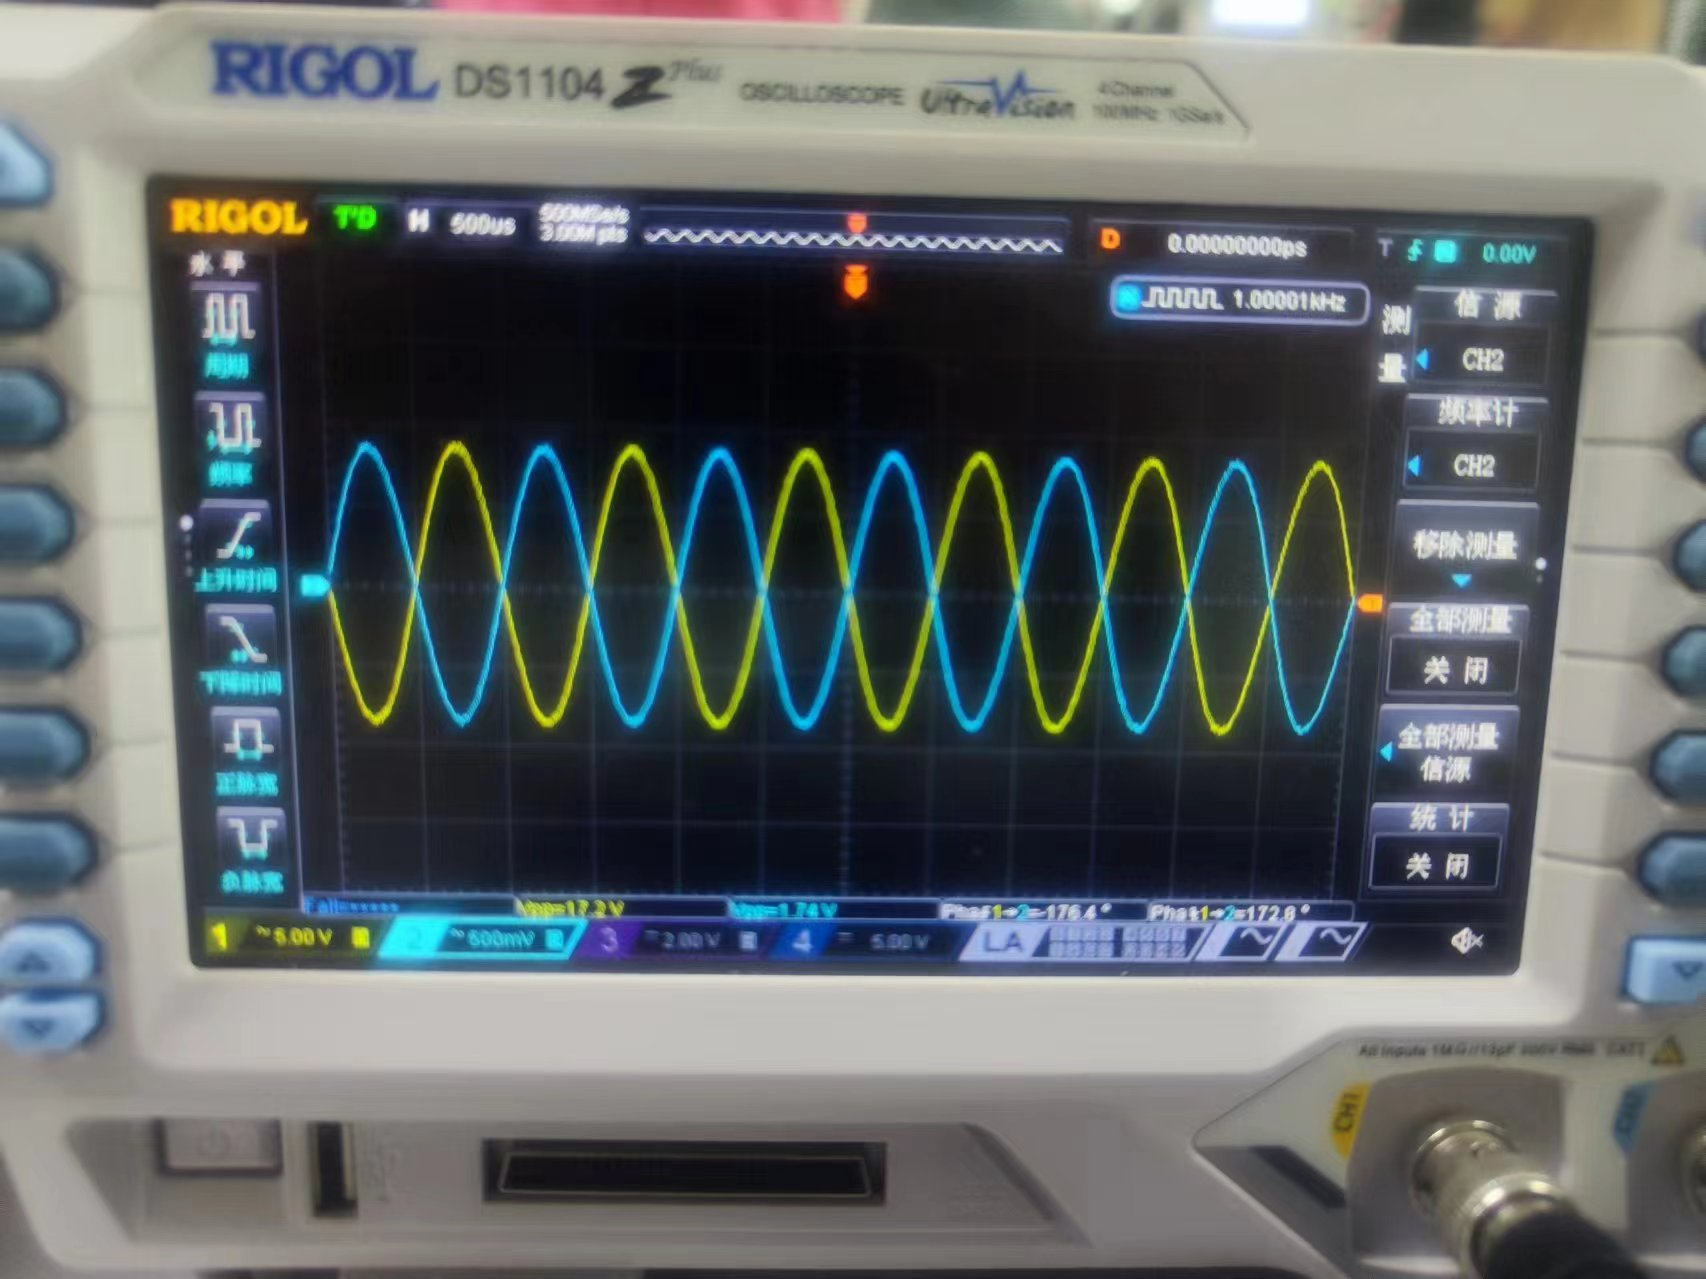
\includegraphics[width=0.6\linewidth]{反相.jpg}
		\caption{反相输出和输入波形}
		\label{}
	\end{figure}
	\subsection{同相比例放大器}
	按图所示连接电路,按给定直流输入信号,测量对应的输出电压,把结果记入表中。
	\begin{table}[!ht]
		\centering
		\begin{tabular}{|l|l|l|l|l|l|l|l|}
		\hline
		Ui(V) & & 0.3 & 0.5 & 0.7 & 1.0 & 1.1 & 1.2 \\ \hline
		理论计算值 & Uo(V) & 3.30 & 5.50 & 7.70 & 11.00 & 12.10 & 13.20 \\ \hline
		实际测量值 & Uo(V) & 3.069 & 5.092 & 7.110 & 10.138 & 11.151 & 12.165 \\ \hline
		实际放大倍数 & Auf & 10.23 & 10.184 & 10.157 & 10.138 & 10.137 & 10.1375 \\ \hline
		\end{tabular}
	\end{table}

	在该比例放大器的输入端加入1KHz, 有效值为0.5V的交流信号,用示波器观察输出波形,并与输入波形相比较。
	\begin{figure}[{H}]
		\centering
		\includegraphics[width=0.6\linewidth]{同相.jpg}
		\caption{同相输出和输入波形}
		\label{}
	\end{figure}
	\subsection{减法器(差分比例运算)}
	按图3连接电路。按给定直流输入信号,测量对应的输出电压,把结果记入表中。
	\begin{table}[H]
		\centering
		\begin{tabular}{|l|l|l|l|}
		\hline
			输入信号Ui1(V) & 0.2 & 0.2 & -0.2  \\ \hline
			  输入信号Ui2 (V) & -0.3 & 0.3 & -0.3  \\ \hline
			计算值Uo (V) &- 5.00& 1.00 & -1.00  \\ \hline
			实际测量值Uo(V) & -5.054 & 1.049 & -1.035  \\ \hline
		\end{tabular}
	\end{table}
	\subsection{反相加法器}
	按图4连接电路。同时将Ui1与Ui2对地短路,接通电源后,调节调零电位器Rp0(10K),使输出Uo=0。然后将短路线去掉,按给定直流输入信号,测量对应的输出电压,把结果记入表中。
	\begin{table}[H]
		\centering
		\begin{tabular}{|l|l|l|l|}
		\hline
			输入信号Ui1(V) & 1.0 & 1.5 & -0.2  \\ \hline
			输入信号Ui2(V) & 0.4 & -0.4 & 1.2  \\ \hline
			计算值Uo(V) &-1.4 & -1.1 &  -1 \\ \hline
			实际测量值Uo(V) &-1.411 & -1.102 &   -1.013\\ \hline
		\end{tabular}
	\end{table}
	\subsection{加减法器}
	按图5连接电路。将3R10与第一级运放的联接断开,按前述方法对两级分别进行调零。然后将短路线去掉,接好电路,按给定直流输入信号(Ui1和Ui2由同一信号源提供),测量对应的输出电压,把结果记入表中。
	\begin{table}[!ht]
		\centering
		\begin{tabular}{|l|l|l|l|l|}
		\hline
			Ui1(V) & Ui2(V) & Ui3(V) & 计算值Uo(V) & 实际测量值Uo(V)  \\ \hline
			0.4 & 0.8 & 0.4 &1
			.02 & 1.075 \\ \hline
		\end{tabular}
	\end{table}
	
	\subsection{实验过程遇到问题及解决办法}
	\begin{enumerate}
		\item 实验中出现了由于错误的连接电路,导致了实验所用芯片烧毁,更换芯片之后,出现了需要调零的问题,所以实验数据是通过手动调零的方式进行记录的。
		\item \textbf{实验的信号发生器的输出的线存在问题,在进行线路排查,数据对比之后,最终确定了信号发生器因为线路没有输出任何信号,在更换输出线之后示波器得到了稳定且正确的图像。}
		\item 在检查实验数据时,老师提出了对于同相放大器的理论值计算问题,这一部分我在实验误差分析部分进行了初步讨论。
	\end{enumerate}
	% ---
	
	
	
	% 分析与讨论	
	\clearpage
	
	% 顶栏
	\begin{table}
		\renewcommand\arraystretch{1.7}
		\begin{tabularx}{\textwidth}{|X|X|X|X|}
			\hline
			专业:& 物理学 &年级:& 2022级\\
			\hline
			姓名: & 黄罗琳、王显 & 学号:&22344001、22344002 \\
			\hline
			日期:& 2024/5/29 & 评分: &\\
			\hline
		\end{tabularx}
	\end{table}
	% ---
	
	% 小标题
	\section{ET11模拟运算放大电路 \quad\heiti 分析与讨论}
	% ---
	
	% 数据处理
	\subsection{描述用示波器观察波形的情况}
	\begin{figure}[H]
		\centering
		\begin{tabular}{cc}
			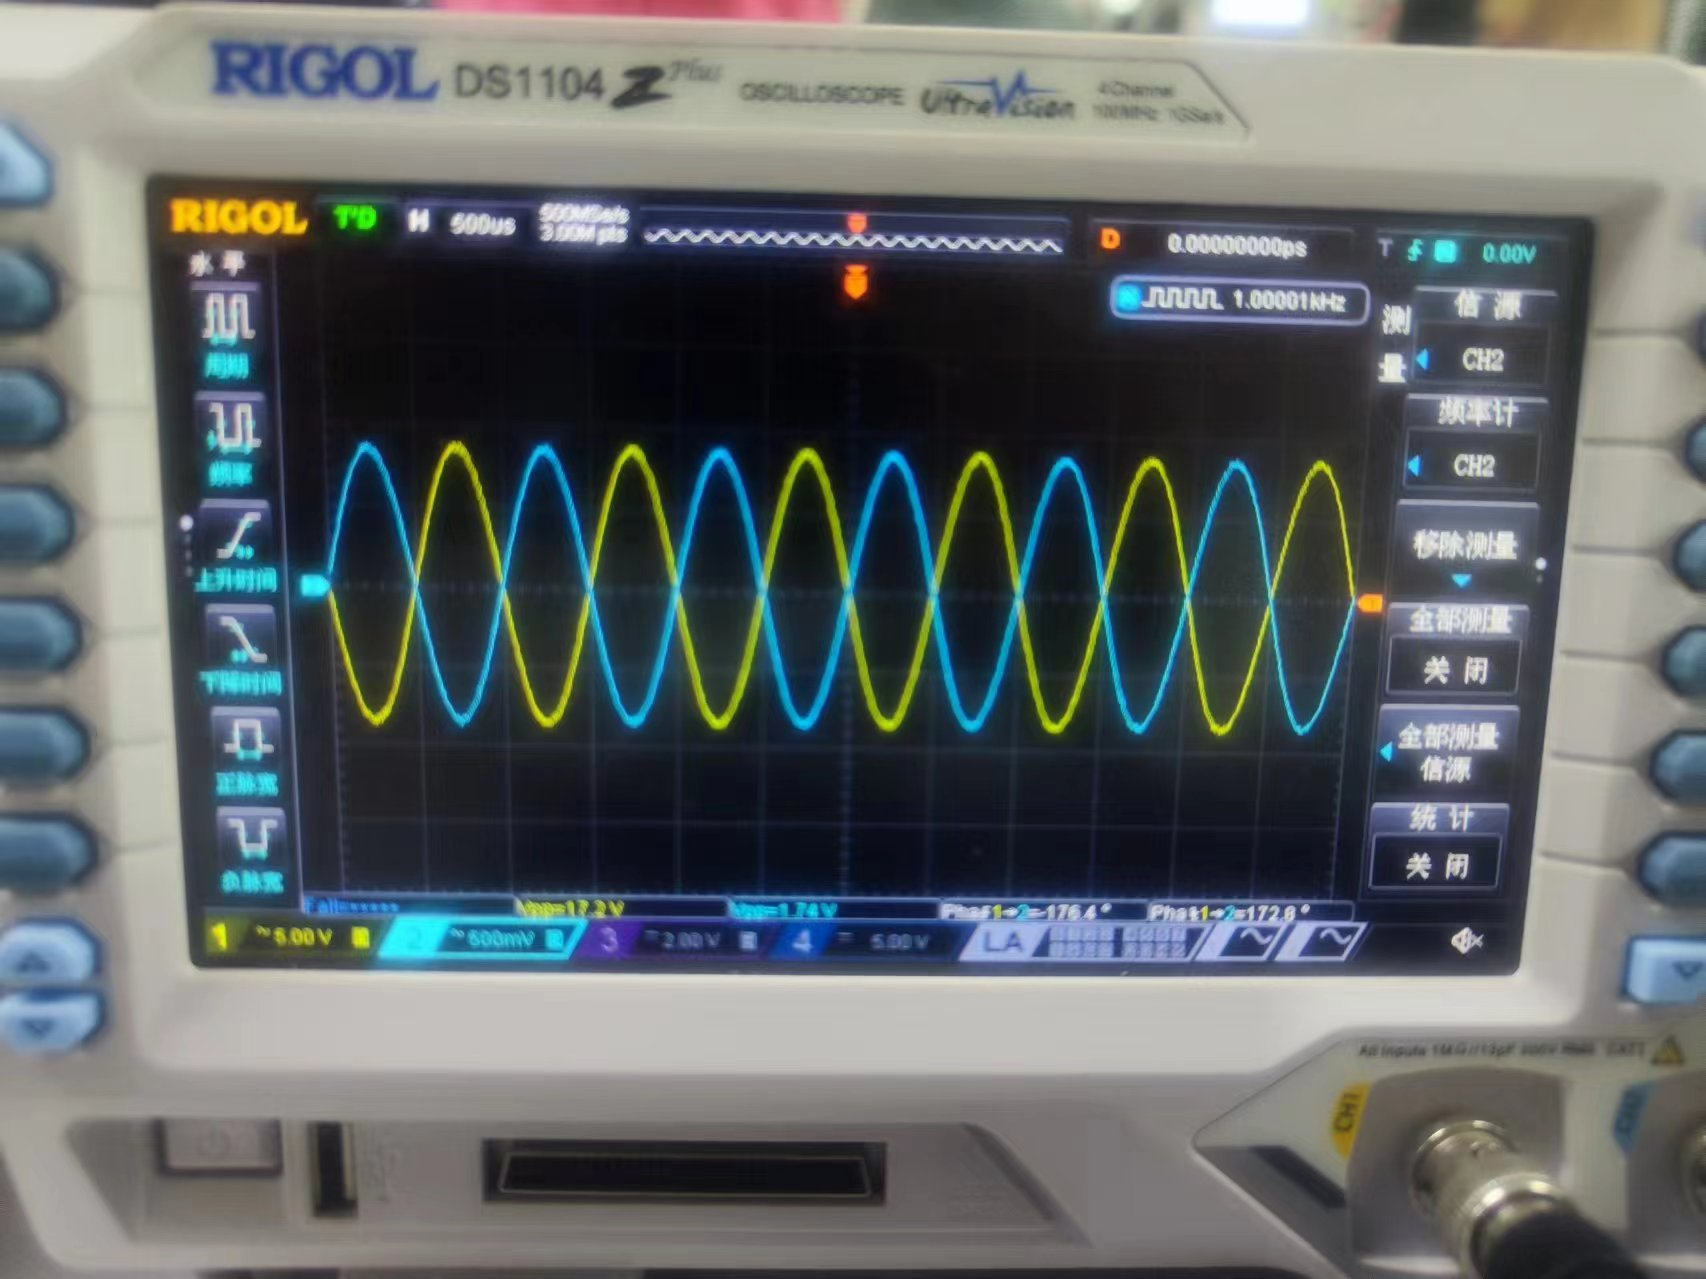
\includegraphics[width=0.5\linewidth]{反相.jpg} & 
			\includegraphics[width=0.5\linewidth]{同相.jpg} \\
			\textbf{(a) 反相输出和输入波形} & \textbf{(b) 同相输出和输入波形}
		\end{tabular}
		\caption{反相和同相输出和输入波形}
		\label{fig:waveforms}
	\end{figure}
	
	反相比例放大器的输出波形与输入波形相比,幅值增大10倍(左下角相差10倍,为5v和500mv),相位相差$\frac{\pi}{2};$

	同相比例放大器的输出波形与输入波形相比,幅值增大10倍,相位相同。
	\subsection{对比理论计算,分析误差}
	理论计算的重点在于,对于同相放大器中对于电压增益的计算。

	根据实验数据

	\begin{table}[!ht]
		\centering
		\begin{tabular}{|l|l|l|l|l|l|l|l|}
		\hline
		Ui(V) & & 0.3 & 0.5 & 0.7 & 1.0 & 1.1 & 1.2 \\ \hline
		理论计算值 & Uo(V) & 3.30 & 5.50 & 7.70 & 11.00 & 12.10 & 13.20 \\ \hline
		实际测量值 & Uo(V) & 3.069 & 5.092 & 7.110 & 10.138 & 11.151 & 12.165 \\ \hline
		实际放大倍数 & Auf & 10.23 & 10.184 & 10.157 & 10.138 & 10.137 & 10.1375 \\ \hline
		\end{tabular}
	\end{table}

	其理论计算值来源于公式
        
      $$A_{uf} = \frac{u_{o}}{u_{i}} = 1 + \frac{R_{f}}{R_{1}}$$
    其主要问题在于,实际上,电路存在电阻分压的问题,故对其放大倍数进行修正,根据实际测量值,其修正公式初步为:

	$$A_{uf}=\frac{u_o}{\frac{10}{11}u_i}$$

	所以修改后的表格为
	
	\begin{table}[!ht]
		\centering
		\begin{tabular}{|l|l|l|l|l|l|l|l|}
		\hline
		Ui(V) & & 0.3 & 0.5 & 0.7 & 1.0 & 1.1 & 1.2 \\ \hline
		理论计算值 & Uo(V) & 3.00 & 5.00 & 7.00 & 10.00 & 12.00 & 13.00 \\ \hline
		实际测量值 & Uo(V) & 3.069 & 5.092 & 7.110 & 10.138 & 11.151 & 12.165 \\ \hline
		实际放大倍数 & Auf & 10.23 & 10.184 & 10.157 & 10.138 & 10.137 & 10.1375 \\ \hline
		\end{tabular}
	\end{table}

	相比于之前的实验数据的误差较小。

	除此之外,实验的数据基本上都误差较小,其误差主要来源可能是,实验电路中引入的电阻导致的实验误差,以及输入电压也可能存在波动,这些都会导致实验最后结果出现误差,但是根据对于理论值和实验值对比发现,这个误差并不是很大,处于可以接受的范围,故认定此次实验较为成功。
	\subsection{实验后思考题}
	
	%思考题1
	\begin{question}
		运算放大器作比例放大时,R1与RF的阻值误差为±10%,试问如何分析和计算电压增益的误差?
	\end{question}
	在运算放大器作比例放大时,电压增益 \( A_{uf} \) 通常表示为:
\[
A_{uf} = -\frac{R_F}{R_1}
\]

假设电阻 \( R_F \) 和 \( R_1 \) 的阻值存在 ±10\% 的误差。

电压增益最大值和最小值

1. \textbf{电阻值的误差范围}:
   \begin{itemize}
       \item \( R_F \) 的取值范围为:\( R_F' = R_F \pm 0.1R_F \),即 \( R_F' \) 可以取 \( 1.1R_F \) 和 \( 0.9R_F \)。
       \item \( R_1 \) 的取值范围为:\( R_1' = R_1 \pm 0.1R_1 \),即 \( R_1' \) 可以取 \( 1.1R_1 \) 和 \( 0.9R_1 \)。
   \end{itemize}

2. \textbf{最大电压增益}:
   电压增益最大值发生在 \( R_F \) 取最大值和 \( R_1 \) 取最小值时:
   \[
   A_{uf}^{\text{max}} = -\frac{1.1R_F}{0.9R_1}
   \]

   对于相对误差:
   \[
   \text{相对误差} = \frac{A_{uf}^{\text{max}} - A_{uf}}{A_{uf}} \times 100\% = \frac{\frac{1.1}{0.9} - 1}{1} \times 100\% = \left( \frac{11}{9} - 1 \right) \times 100\% = \frac{2}{9} \times 100\% \approx 22.2\%
   \]

3. \textbf{最小电压增益}:
   电压增益最小值发生在 \( R_F \) 取最小值和 \( R_1 \) 取最大值时:
   \[
   A_{uf}^{\text{min}} = -\frac{0.9R_F}{1.1R_1}
   \]

   对于相对误差:
   \[
   \text{相对误差} = \frac{A_{uf}^{\text{min}} - A_{uf}}{A_{uf}} \times 100\% = \frac{\frac{0.9}{1.1} - 1}{1} \times 100\% = \left( \frac{9}{11} - 1 \right) \times 100\% = \frac{-2}{11} \times 100\% \approx -18.2\%
   \]
	% 思考题2
	\begin{question}
		运算放大器作精密放大时,同相输入端对地的直流电阻要与反相输入端对地的直流电阻相等,如果不相等,
会引起什么现象?
	\end{question}
	在运算放大器中,同相输入端对地的直流电阻 \( R_{in+} \) 和反相输入端对地的直流电阻 \( R_{in-} \) 如果不相等,会导致以下现象:

1. 偏置电流不同

运算放大器的同相输入端和反相输入端都存在一个偏置电流 \( I_B \),它们通过对地的直流电阻 \( R_{in+} \) 和 \( R_{in-} \) 进行偏置。

假设偏置电流分别为 \( I_{B+} \) 和 \( I_{B-} \),则输入端产生的偏置电压分别为:
\[ V_{in+} = I_{B+} \cdot R_{in+} \]
\[ V_{in-} = I_{B-} \cdot R_{in-} \]

2. 输出信号偏移

输出信号 \( V_{out} \) 受到输入差模电压 \( V_{in+} - V_{in-} \) 的影响,其表达式为:
\[ V_{out} = A \cdot (V_{in+} - V_{in-}) \]

其中, \( A \) 是运算放大器的开环增益。

如果 \( R_{in+} \neq R_{in-} \),则 \( V_{in+} \) 和 \( V_{in-} \) 之间的差异会引起非零的输入差模电压 \( V_{in+} - V_{in-} \),从而导致输出电压 \( V_{out} \) 的偏移。

即使偏置电流 \( I_B \) 很小,输出端的偏移量仍然可以显著影响系统的性能和准确性。为了避免这种偏移,需要确保同相输入端对地的直流电阻 \( R_{in+} \) 和反相输入端对地的直流电阻 \( R_{in-} \) 相等。

	\clearpage
	
	% 小标题
	\section{ET11 运算放大器\quad\heiti 结语}
	% ---
	
	% 总结、杂谈与致谢
	\subsection{实验心得和体会、意见建议等}
	\begin{enumerate}
		\item 实验总体难度不大,但是在实验过程中我们通过控制变量法排查出了线路问题,从而获得了正确的实验图像。
		\item \textbf{本实验报告采用LATEX编辑,实验分工为黄罗琳同学负责记录数据、编辑报告、数据分析,王显同学负责实验操作、误差分析。}
	\end{enumerate}
	% ---
	

	% 附件
	\subsection{附件及实验相关的软硬件资料等} 
	\begin{figure}[{H}]
		\centering
		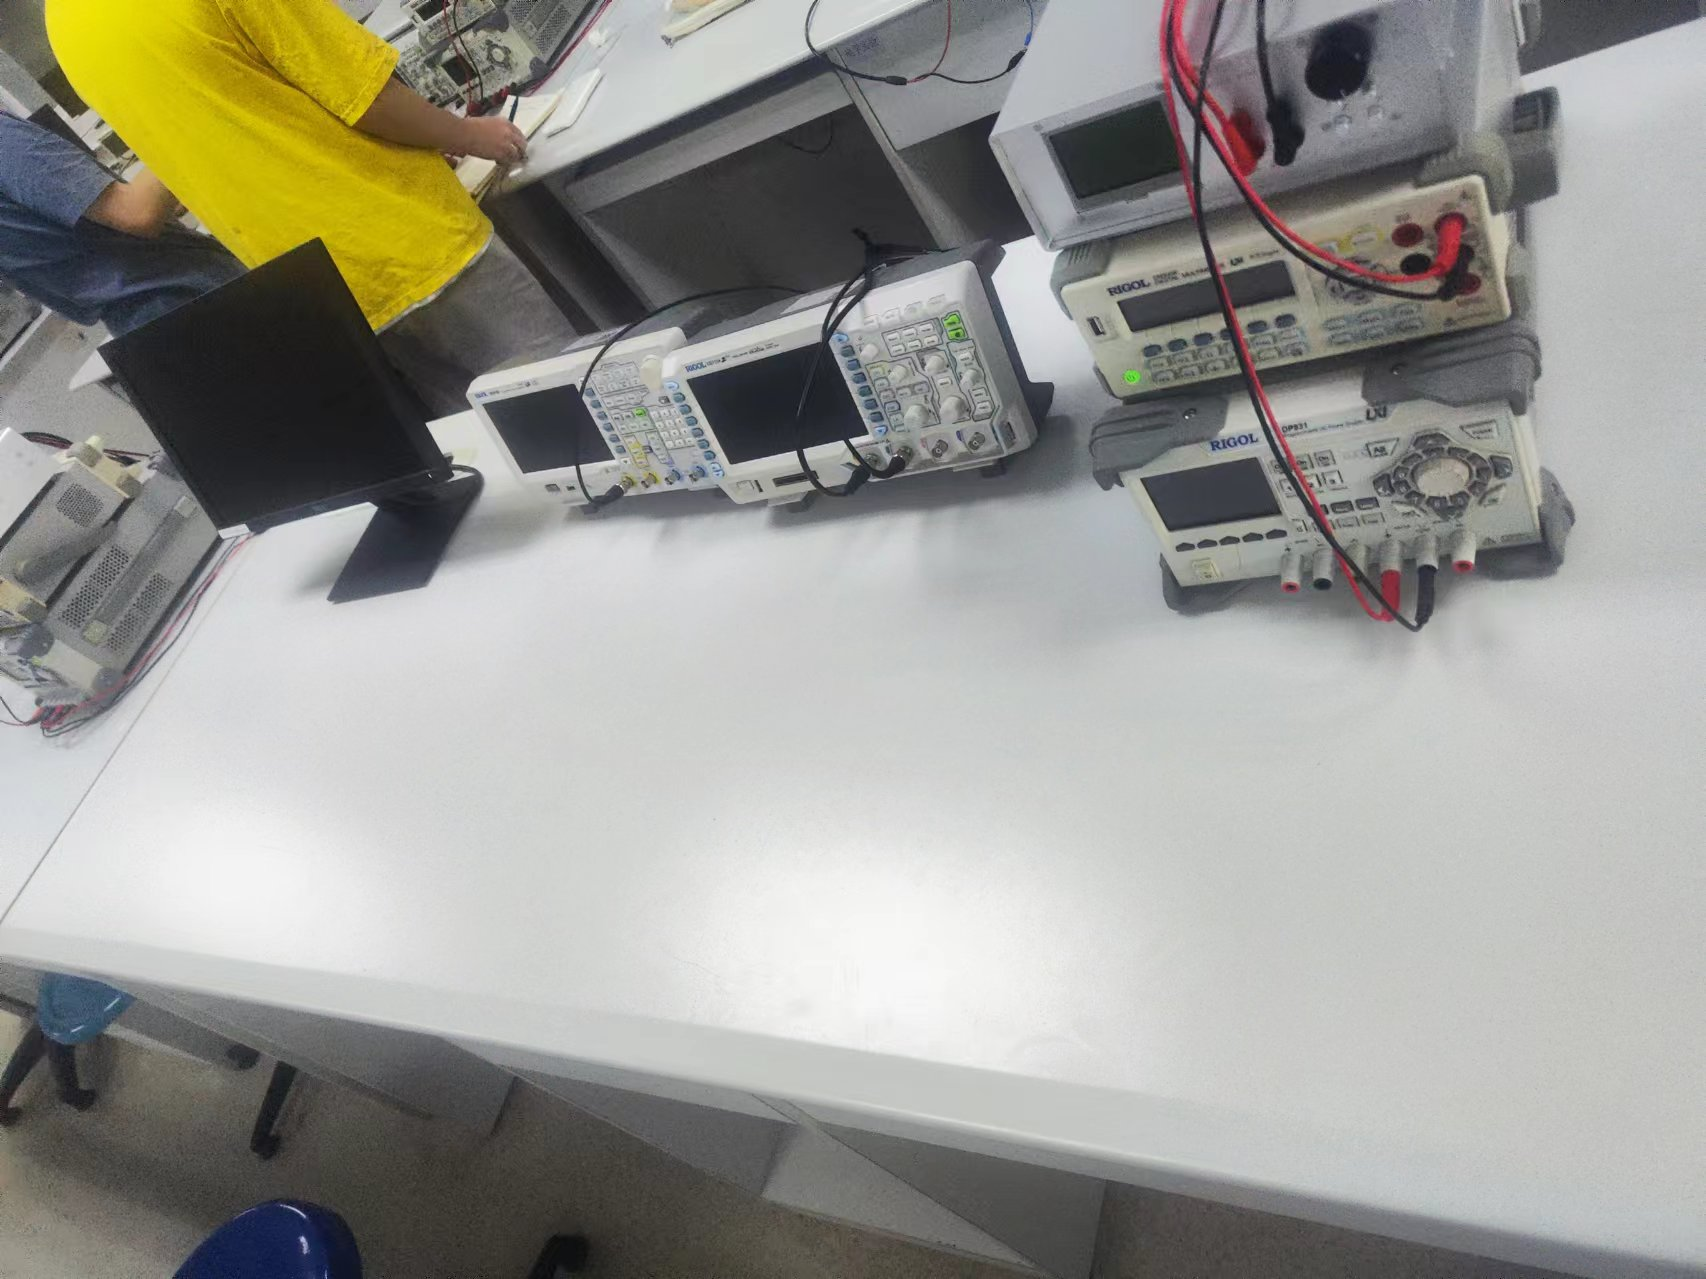
\includegraphics[width=0.4\linewidth]{桌面.jpg}
	\end{figure}
	\begin{figure}[{H}]
		\centering
		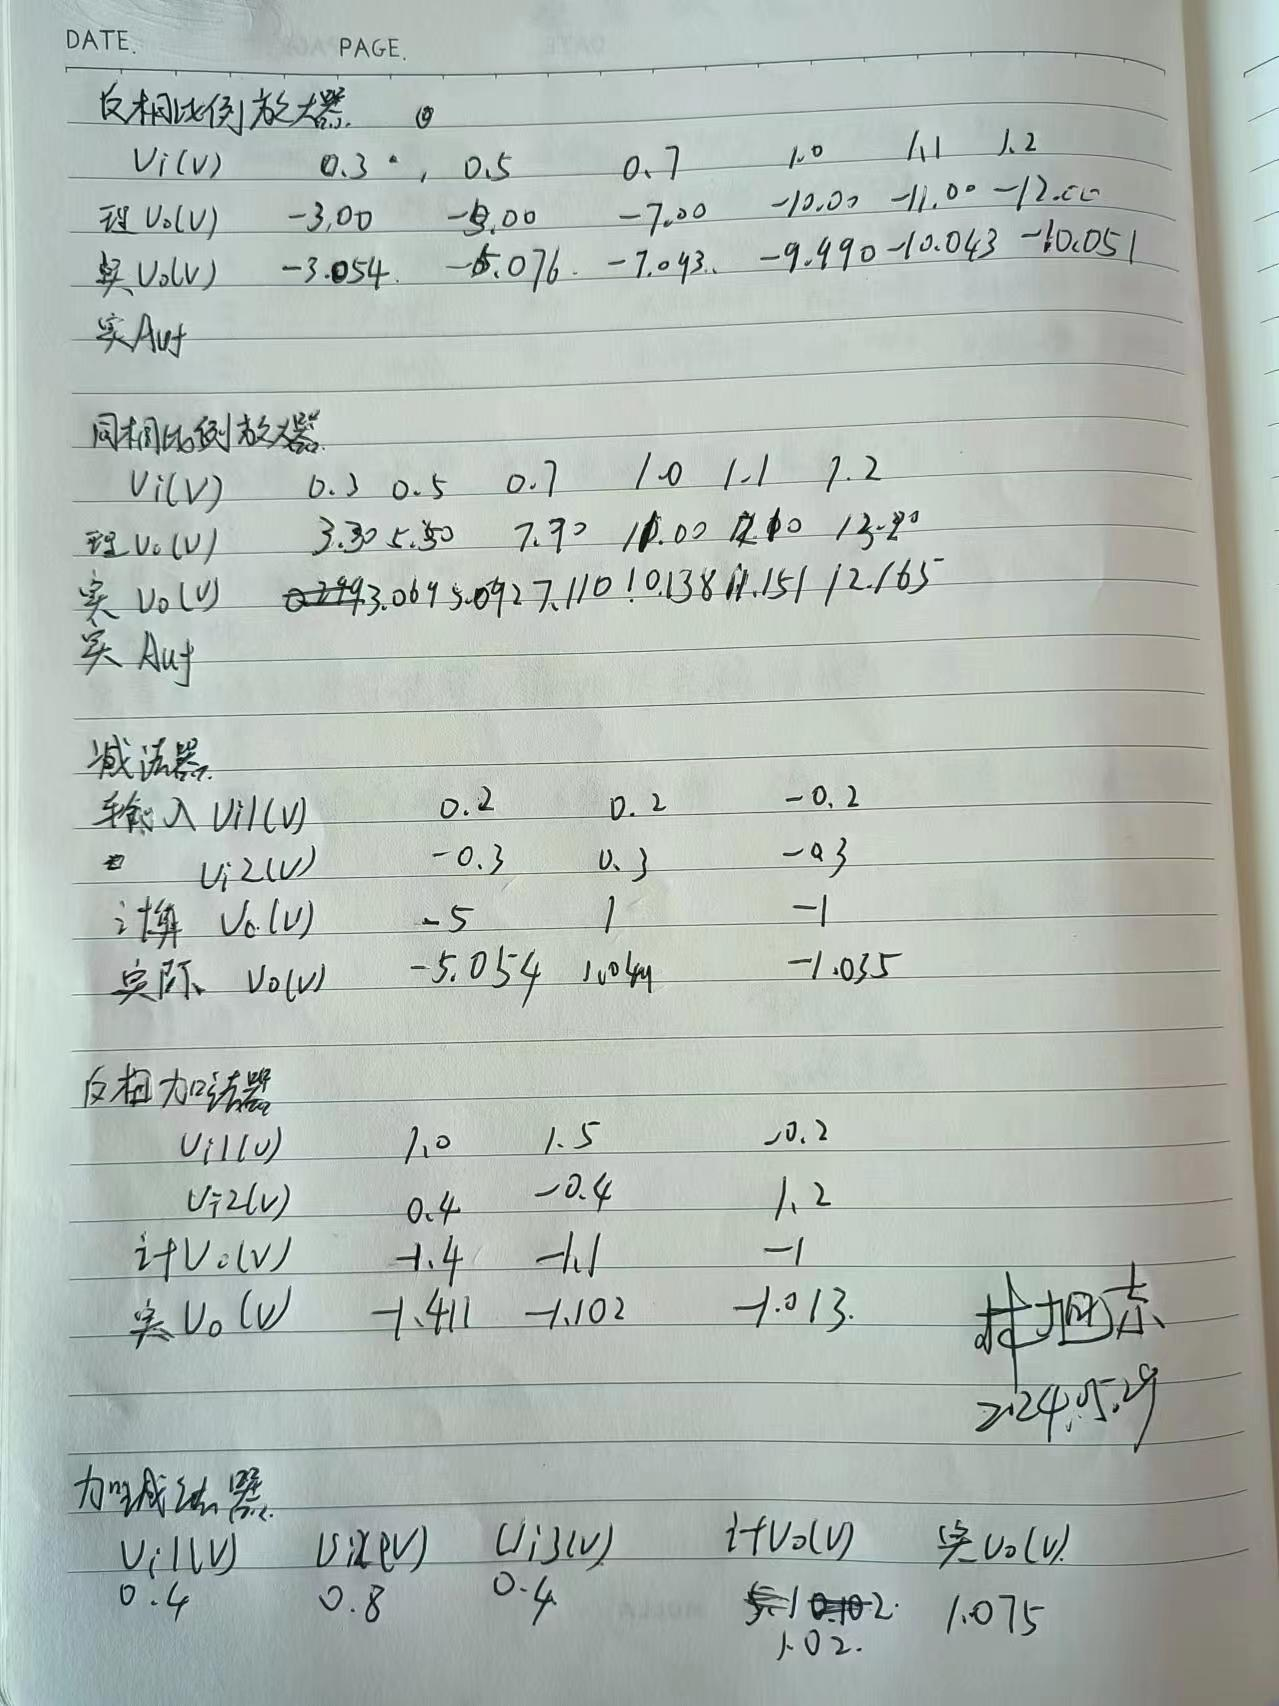
\includegraphics[width=0.4\linewidth]{数据.jpg}
		\caption{实验数据}
		\label{}
	\end{figure}

	% ---
	
	
\end{document}